\chapter{LSST}
\label{chapter:future}

\begin{abstract}
The Large Synoptic Survey Telescope (\LSST) will provide sparse but precise
ground-based photometry for billions of field and cluster cool dwarfs.
We explore {\it LSST}’s potential for large-scale rotation period measurement
with an emphasis on applications to gyrochronology, the method of inferring
stellar ages from rotation periods.
With its ten year baseline, \LSST\ light curves will be sensitive to long
rotation periods which are characteristic of old and low-mass stars.
New asteroseismic data from the \kepler\ spacecraft have revealed that
magnetic braking may cease at around Solar Rossby number, implying that
gyrochronology is not applicable to old stars.
By measuring rotation periods of old, slowly rotating, low-mass stars we can
decisively test the age-rotation relations at all ages.
Of particular interest are the open clusters with precisely measured
isochronal ages.
These clusters will allow us to recalibrate the age-rotation relations in the
old, low-mass regime, provided we can measure the photometric rotation periods
of their members.
Using representative distributions of stellar ages and spectral types from
\TRILEGAL outputs, we simulated thousands of light curves using a
gyrochronology relation, a simple star-spot model and approximate \LSST\
cadence.
By running a rotation period recovery pipeline, we predict the number of
accurately measured cool dwarf rotation periods expected from \LSST\ as a
function of spectral type, magnitude and rotation period.
Using the full ten-year data set we are able to accurately recover 60-70\% of
rotation periods for stars with $T_{\mathrm{eff}}>4500$ K and 70-80\% for
stars with $T_{\mathrm{eff}}<4500$ K, brighter than 23rd magnitude.

\end{abstract}

\section{Introduction}

The Large Synoptic Survey Satellite (\LSST) is a 8.4 metre telescope with a
9.6 square degree field of view in Cerro Pach\'{o}n, Chile, currently under
construction.
It is designed to observe 18,000 square degrees in the southern sky (south of
+10 degrees, declination) in six Sloan Digital Sky Survey (\SDSS) filters:
{\it ugrizy}.
During its main mode of operation (90\% of the time), \LSST\ will perform two
fifteen second exposures per visit, with one thousand visits per night and
will have a faint limit of around 24.5 in r-band.
For the remaining 10\% of the time, \LSST\ will focus on a small number of
`deep drilling fields'.
These fields are yet to be determined but could be, for example, the Large and
Small Magellanic Clouds, the galactic plane, and so on.
These fields will receive targeted, repeat observations of, for instance 200
observations over a 40-hour period after which the faint limit could be
extended to around 28 apparent magnitudes.
First light is currently scheduled for 2021 and data release one of eleven is
expected to contain eighteen billion objects \citep{Ivezic2008}.

\LSST\ will provide photometric rotation periods for a new region of
period-mass-age parameter space.
The \kepler\ spacecraft focused on Earth-like planets with Sun-like hosts,
thus the majority of its targets were G type, with fewer K and M dwarfs.
Unlike \kepler\ however, any target falling within \LSST's field of view will
be observed --- not just those on a predetermined target list.
In addition, due to the large collecting area of \LSST, it will be sensitive
to a large number of faint stars, including many K and M dwarfs.
Being ground-based, its lifetime does not depend on the reliability of moving
parts or fuel and \LSST\ will run for 10 years, more than double the length of
the \kepler\ prime mission.
This long baseline will enable rotation signatures of faint, slowly rotating
stars to be detected, populating both low-mass and old regions of the
age-rotation parameter space.
\LSST\ will provide an extremely different but complementary data set to
\kepler: whereas \kepler\ data are dense and evenly spaced, \LSST\ light
curves will have sparse, irregular cadence.
Despite the sparcity of \LSST\ data, its irregular cadence will extend the
minimum recoverable period limit.
With the exception of the deep drilling fields, the minimum interval
between exposures will be around three days for the majority of targets.
This corresponds to a nominal minimum recoverable period of around six days,
however, the irregularity of \LSST\ cadence, combined with the ten year
observing window will reduce this lower bound.

In order to investigate the potential of \LSST\ data regarding gyrochronology,
it is essential that we estimate the range of rotation periods that will be
detectable.
In what follows we describe our \LSST-like, simulated data-set and our
rotation period recovery pipeline.

\section{Simulations}
We developed a simple \LSST\ cadence model for our simulations\footnote{In
future we intend to use the \LSST\ operations simulator (OpSim) to generate a
more realistic cadence pattern for each target, depending on its position on
the sky.}.
This model generates a cadence pattern for each object by requiring that it
only be observed during the night and whilst that field is visible, \ie\ for
half of the year.
Each object is visited every three days on average during the observable
season and visits are clustered around a season with a Gaussian shape.
A histogram of the number of visits per week as a function of time for a given
object or field is shown in figure \ref{fig:cadence_hist}.
The code used to simulate \LSST\ cadence was written by J. Davenport and is
available at \url{https://github.com/jradavenport/MW-Flare}.

\begin{figure}
\begin{center}
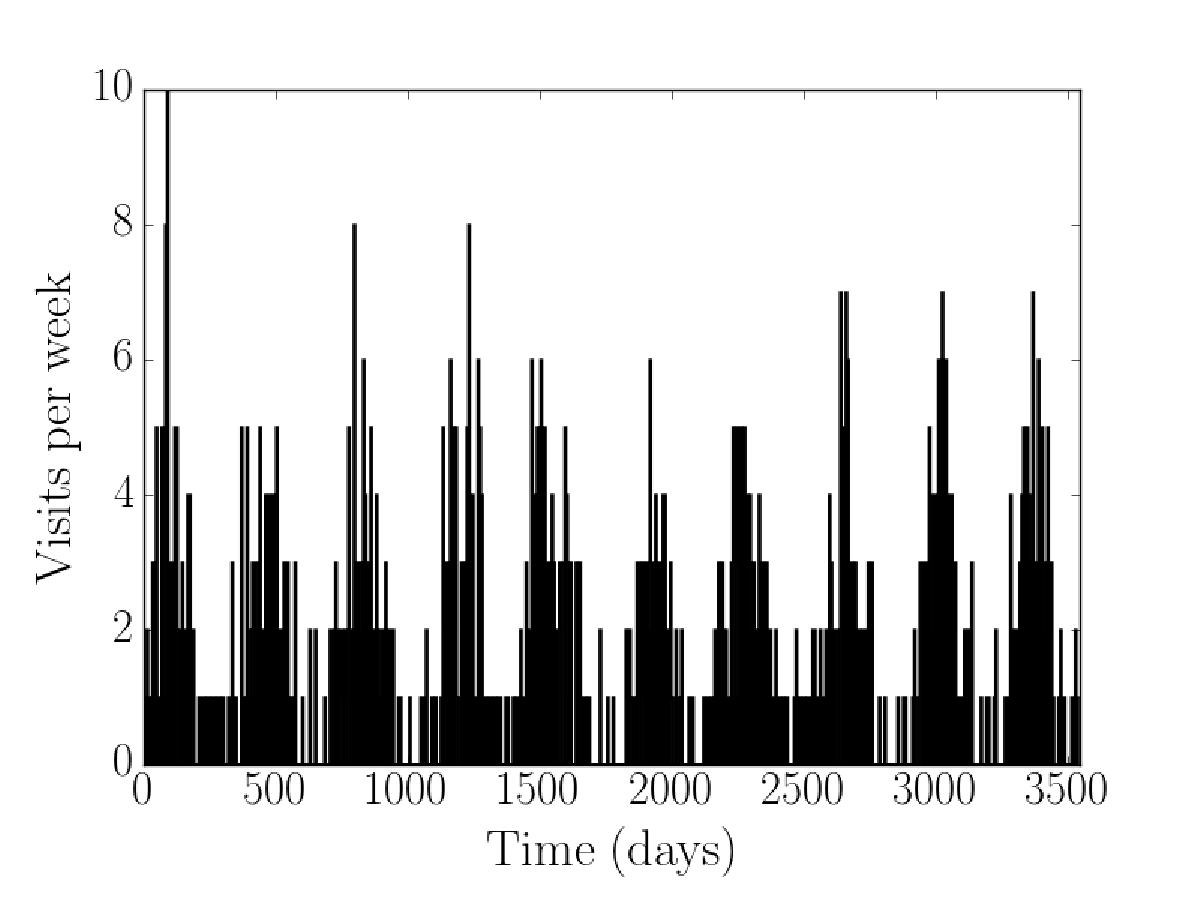
\includegraphics[width=6in, clip=true]{figures/cadence_hist}
\caption[An \LSST\ cadence histogram.]
{A histogram of the number of visits per week as a function of time
for a given object or field observed by \LSST\ as used in our simulations.
Each object is observed only during the day and for half a year at a time.
The code used to generate this plot was written by J. Davenport,
\url{https://github.com/jradavenport/MW-Flare}.}
\label{fig:cadence_hist}
\end{center}
\end{figure}

\subsection{Field stars}
We used the \TRILEGAL\ \citep{Girardi2012} galaxy simulation code to generate
field stellar populations for two hypothetical \LSST\ fields.
These fields were centred on the same galactic longitude, $l=45$, but
different galactic longitude: one close to the galactic plane, $b=-20$ and one
slightly out of the plane, $b=-60$.
\TRILEGAL\ takes the coordinates and size of a field within the galaxy as
inputs and simulates the population of stars in that field.
It returns a catalogue of simulated stars with their properties: age,
effective temperature and $ugriz$ magnitudes, and others.
We randomly selected 20,000 stars from each field in order to produce a
representative but manageable target sample.
Selected stars had $r$-band magnitudes between 16 and 28 and \logg $>4$.
These target stars were then separated into `cool' ($T_{\mathrm{eff}}< 6250$)
and `hot' ($6250 < T_{\mathrm{eff}}$) temperature bins.
Rotation periods for the cool stars were calculated using the
\citet{Angus2015} gyrochronology relation which converts \TRILEGAL\ ages and
$B-V$ colour (calculated from \TRILEGAL\ $g-r$) into rotation periods.
Hot stars ($T_{\mathrm{eff}}\gtrsim 6250$) lack a significant convective
envelope.
Since the combination of convective plasma motion and stellar rotation is
responsible for magnetic field generation, these stars do not undergo magnetic
braking.
As such, their rotation periods cannot be estimated using gyrochronology.
To assign rotation periods to the hot stars we fitted a sum of two Gaussian
functions to the rotation periods of hot stars in the \citet{Mcquillan2014}
catalogue and randomly sampled from the resulting distribution.
The distribution of hot star rotation periods is shown in figure
\ref{fig:hot_star_hist}.

\begin{figure}
\begin{center}
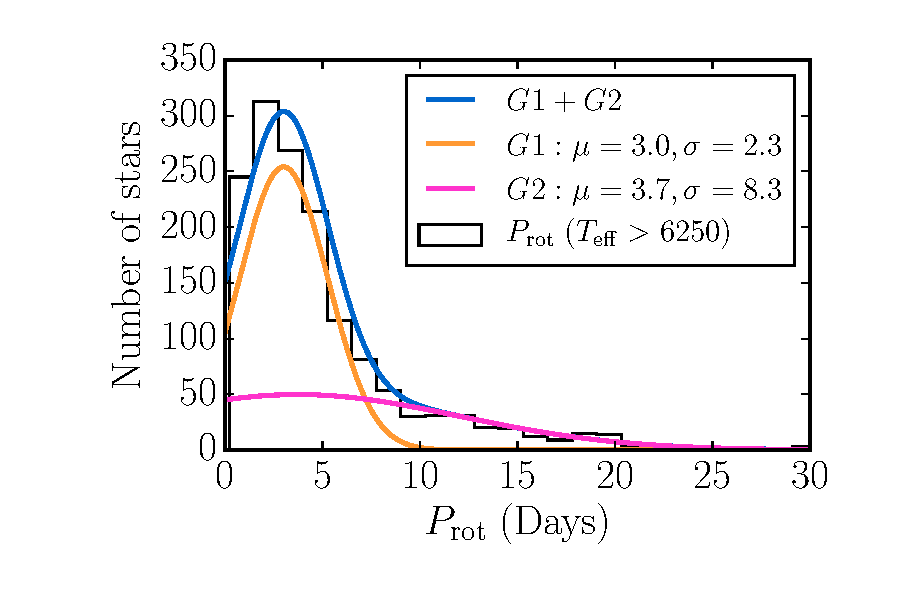
\includegraphics[width=6in, clip=true]{figures/hot_star_hist.pdf}
\caption[A histogram of the rotation periods of hot stars from
\citet{Mcquillan2014}.]
{A histogram of the rotation periods of stars with $T_{\mathrm{eff}} > 6250$K
from the \citet{Mcquillan2014} catalogue.
We fit a sum of two Gaussians to this distribution in order to assign rotation
periods to the hot stars in our \trilegal samples.}
\label{fig:hot_star_hist}
\end{center}
\end{figure}

\subsection{Cluster stars}
In addition to field stars, we simulated light curves for hypothetical members
of three open clusters: IC 4651 (1778 Myr), NGC 5316 (170 Myr) and NGC 2477
(822 Myr).
Representative numbers of G dwarfs in each cluster were estimated from
previously published CMDs.
Numbers of K and M dwarfs were then estimated using the \citet{Kroupa2001}
initial mass function (IMF).
Metallicities, distances, reddening, and ages were obtained from the
\citet{Kharchenko2013} catalogue.
In order to calculate theoretical rotation periods for stars in these
clusters, we used three broad temperature bins, corresponding to the three
spectral types: $G$, $K$ and $M$.
$G$ type was defined as $5200 < T_{\mathrm{eff}} < 6000$ K, $K$ as $3700 <
T_{\mathrm{eff}} < 5200$ and $M$ as $2400 < T_{\mathrm{eff}} < 5200$.
Cluster member catalogues were simulated by randomly drawing effective
temperatures from uniform distributions bounded by these limits.
This is a relatively crude way to simulate cluster member temperatures, and an
improved approach would be to use an IMF.
We hope to modify our method in future in order to quantify rotation period
recoverability as a function of effective temperature rather than spectral
type.
$B-V$ colours were estimated for cluster members using the
\citet{Sekiguchi2000} relation for $B-V$, temperature, metallicity and
\logg\footnote{We used Solar \logg\ for all spectral types.}, and reddening.
$r$-band magnitudes were then approximated using $B-V$ colour and approximate
V-band apparent magnitudes for each spectral type in each cluster.
We generated 2000 each of $G$, $K$ and $M$ dwarfs for all three clusters:
18,000 stars in total.
We simulated equal numbers of G, K and M spectral types, rather than
representative relative numbers in order to adequately sample the entire
range of temperature space.
Using representative numbers would provide excellent M dwarf but very poor G
dwarf coverage.
Rotation periods were calculated for the theoretical cluster members using the
\citet{Angus2015} gyrochronology relation.

\subsection{Synthesising light curves}
Once theoretical rotation periods had been assigned to both hot and cool field
and cluster stars we used code similar to that used in \citet{Aigrain2015b} to
simulate light curves.
These light curves are calculated by placing dark spots on a rotating sphere
and integrating the total resulting flux over the surface.
Stellar flux variations produced by dark active regions on the surface are
typically non-sinusoidal and this simple spot model provides a more accurate
representation of stellar light curves than a simple sinusoid.
However, it should be noted that this code can be adjusted to produce more
realistic light curves by altering spot lifetimes and including differential
rotation with spot migration.
Stars with spot lifetimes that are short relative to their rotation periods
will display quasi-periodic brightness variations in their light curves.
Including differential rotation will compound this effect and further perturb
star spot light curve features from strict periodicity.
We fixed the mean spot lifetime at 30.5 days for all simulations and did not
include differential rotation.
For this reason, our simulated light curves are highly periodic, with only
small deviations from strict periodicity.
Rotation periods are more easy to recover from strictly periodic light curves
than for quasi-periodic ones and for this reason, our results should be
considered `best case'.
In future we plan to vary spot lifetimes and include differential rotation in
our spot model in order to produce more realistic light curves.

In order to assign appropriate amplitudes to the simulated light curves we
approximated the relation between rotation period, amplitude of variability
and \teff, based on the \citet{Mcquillan2014} sample.
We then assigned amplitudes by drawing values from Gaussians with means
corresponding to the mean amplitudes of stars with similar \teff\ and
$P_{rot}$ in \citet{Mcquillan2014} and variances given by the variance in each
bin.
White noise was added to the light curves, with amplitudes that depended on
$r$-band magnitude, based on the values provided in \citet{Jacklin2015}.
We sampled these light curves using our \LSST\ cadence model and attempted to
recover their rotation periods using a Lomb-Scargle (LS) periodogram
\citep[][]{Lomb1976, Scargle1982}.
LS periodograms were computed for each light curve over a grid of 1000 periods
ranging from 2 to 100 days.
The position of the highest peak in the periodogram was recorded as the
measured period.

An LS periodogram is not ideal for measuring rotation periods from stellar
light curves because star spots tend to produce non-sinusiodal, quasi-periodic
brightness variations.
A commonly used alternative to the LS periodogram is the auto-correlation
function (ACF) which is better suited to non-sinusoidal, quasi-periodic
signals, as demonstrated by \citet{Mcquillan2013}.
previous chapters,
Unfortunately however, evenly spaced data are required to produce an ACF.
Another alternative method that has produced promising results using Gaussian
processes (GPs) is currently under development \citep{Angus2015b}, however it
is relatively computationally expensive.
We have used the LS periodogram in these initial tests because it is fast to
compute, but intend to use the GP method in the future.

% references:

% @ARTICLE{Jacklin2015,
%    author = {{Jacklin}, S. and {Lund}, M.~B. and {Pepper}, J. and {Stassun}, K.~G.
% 	},
%     title = "{Transiting Planets with LSST. II. Period Detection of Planets Orbiting 1 M$_{⊙}$ Hosts}",
%   journal = {\aj},
% archivePrefix = "arXiv",
%    eprint = {1503.00059},
%  primaryClass = "astro-ph.EP",
%  keywords = {planets and satellites: detection, planets and satellites: general, surveys},
%      year = 2015,
%     month = jul,
%    volume = 150,
%       eid = {34},
%     pages = {34},
%       doi = {10.1088/0004-6256/150/1/34},
%    adsurl = {http://adsabs.harvard.edu/abs/2015AJ....150...34J},
%   adsnote = {Provided by the SAO/NASA Astrophysics Data System}
% }

% @ARTICLE{Kroupa2001,
%    author = {{Kroupa}, P.},
%     title = "{On the variation of the initial mass function}",
%   journal = {\mnras},
%    eprint = {astro-ph/0009005},
%  keywords = {BINARIES: GENERAL, STARS: FORMATION, STARS: KINEMATICS, STARS: LUMINOSITY FUNCTION, MASS FUNCTION, GLOBULAR CLUSTERS: GENERAL, OPEN CLUSTERS AND ASSOCIATIONS: GENERAL},
%      year = 2001,
%     month = apr,
%    volume = 322,
%     pages = {231-246},
%       doi = {10.1046/j.1365-8711.2001.04022.x},
%    adsurl = {http://adsabs.harvard.edu/abs/2001MNRAS.322..231K},
%   adsnote = {Provided by the SAO/NASA Astrophysics Data System}
% }

% @ARTICLE{Kharchenko2013,
%    author = {{Kharchenko}, N.~V. and {Piskunov}, A.~E. and {Roeser}, S. and
% 	{Schilbach}, E. and {Scholz}, R.-D.},
%     title = "{VizieR Online Data Catalog: Milky Way global survey of star clusters. II. (Kharchenko+, 2013)}",
%   journal = {VizieR Online Data Catalog},
%  keywords = {Clusters: open, Radial velocities, Proper motions, Milky Way},
%      year = 2013,
%     month = nov,
%    volume = 355,
%    adsurl = {http://adsabs.harvard.edu/abs/2013yCat..35580053K},
%   adsnote = {Provided by the SAO/NASA Astrophysics Data System}
% }

% @ARTICLE{Angus2015,
%    author = {{Angus}, R. and {Aigrain}, S. and {Foreman-Mackey}, D. and {McQuillan}, A.
% 	},
%     title = "{Calibrating gyrochronology using Kepler asteroseismic targets}",
%   journal = {\mnras},
% archivePrefix = "arXiv",
%    eprint = {1502.06965},
%  primaryClass = "astro-ph.EP",
%  keywords = {methods: statistical, stars: evolution, stars: fundamental parameters, stars: oscillations, stars: rotation, stars: solar-type},
%      year = 2015,
%     month = jun,
%    volume = 450,
%     pages = {1787-1798},
%       doi = {10.1093/mnras/stv423},
%    adsurl = {http://adsabs.harvard.edu/abs/2015MNRAS.450.1787A},
%   adsnote = {Provided by the SAO/NASA Astrophysics Data System}
% }

% @ARTICLE{Angus2015b,
%    author = {{Angus}, R. and {Aigrain}, S. and {Foreman-Mackey}, D.},
%     title = "{Probabilistic stellar rotation periods with Gaussian processes}",
%   journal = {IAU General Assembly},
%      year = 2015,
%     month = aug,
%    volume = 22,
%       eid = {2258396},
%     pages = {2258396},
%    adsurl = {http://adsabs.harvard.edu/abs/2015IAUGA..2258396A},
%   adsnote = {Provided by the SAO/NASA Astrophysics Data System}
% }

% @ARTICLE{Ivezic2008,
%    author = {{Ivezic}, Z. and {Tyson}, J.~A. and {Abel}, B. and {Acosta}, E. and
% 	{Allsman}, R. and {AlSayyad}, Y. and {Anderson}, S.~F. and {Andrew}, J. and
% 	{Angel}, R. and {Angeli}, G. and {Ansari}, R. and {Antilogus}, P. and
% 	{Arndt}, K.~T. and {Astier}, P. and {Aubourg}, E. and {Axelrod}, T. and
% 	{Bard}, D.~J. and {Barr}, J.~D. and {Barrau}, A. and {Bartlett}, J.~G. and
% 	{Bauman}, B.~J. and {Beaumont}, S. and {Becker}, A.~C. and {Becla}, J. and
% 	{Beldica}, C. and {Bellavia}, S. and {Blanc}, G. and {Blandford}, R.~D. and
% 	{Bloom}, J.~S. and {Bogart}, J. and {Borne}, K. and {Bosch}, J.~F. and
% 	{Boutigny}, D. and {Brandt}, W.~N. and {Brown}, M.~E. and {Bullock}, J.~S. and
% 	{Burchat}, P. and {Burke}, D.~L. and {Cagnoli}, G. and {Calabrese}, D. and
% 	{Chandrasekharan}, S. and {Chesley}, S. and {Cheu}, E.~C. and
% 	{Chiang}, J. and {Claver}, C.~F. and {Connolly}, A.~J. and {Cook}, K.~H. and
% 	{Cooray}, A. and {Covey}, K.~R. and {Cribbs}, C. and {Cui}, W. and
% 	{Cutri}, R. and {Daubard}, G. and {Daues}, G. and {Delgado}, F. and
% 	{Digel}, S. and {Doherty}, P. and {Dubois}, R. and {Dubois-Felsmann}, G.~P. and
% 	{Durech}, J. and {Eracleous}, M. and {Ferguson}, H. and {Frank}, J. and
% 	{Freemon}, M. and {Gangler}, E. and {Gawiser}, E. and {Geary}, J.~C. and
% 	{Gee}, P. and {Geha}, M. and {Gibson}, R.~R. and {Gilmore}, D.~K. and
% 	{Glanzman}, T. and {Goodenow}, I. and {Gressler}, W.~J. and
% 	{Gris}, P. and {Guyonnet}, A. and {Hascall}, P.~A. and {Haupt}, J. and
% 	{Hernandez}, F. and {Hogan}, C. and {Huang}, D. and {Huffer}, M.~E. and
% 	{Innes}, W.~R. and {Jacoby}, S.~H. and {Jain}, B. and {Jee}, J. and
% 	{Jernigan}, J.~G. and {Jevremovic}, D. and {Johns}, K. and {Jones}, R.~L. and
% 	{Juramy-Gilles}, C. and {Juric}, M. and {Kahn}, S.~M. and {Kalirai}, J.~S. and
% 	{Kallivayalil}, N. and {Kalmbach}, B. and {Kantor}, J.~P. and
% 	{Kasliwal}, M.~M. and {Kessler}, R. and {Kirkby}, D. and {Knox}, L. and
% 	{Kotov}, I. and {Krabbendam}, V.~L. and {Krughoff}, S. and {Kubanek}, P. and
% 	{Kuczewski}, J. and {Kulkarni}, S. and {Lambert}, R. and {Le Guillou}, L. and
% 	{Levine}, D. and {Liang}, M. and {Lim}, K. and {Lintott}, C. and
% 	{Lupton}, R.~H. and {Mahabal}, A. and {Marshall}, P. and {Marshall}, S. and
% 	{May}, M. and {McKercher}, R. and {Migliore}, M. and {Miller}, M. and
% 	{Mills}, D.~J. and {Monet}, D.~G. and {Moniez}, M. and {Neill}, D.~R. and
% 	{Nief}, J. and {Nomerotski}, A. and {Nordby}, M. and {O'Connor}, P. and
% 	{Oliver}, J. and {Olivier}, S.~S. and {Olsen}, K. and {Ortiz}, S. and
% 	{Owen}, R.~E. and {Pain}, R. and {Peterson}, J.~R. and {Petry}, C.~E. and
% 	{Pierfederici}, F. and {Pietrowicz}, S. and {Pike}, R. and {Pinto}, P.~A. and
% 	{Plante}, R. and {Plate}, S. and {Price}, P.~A. and {Prouza}, M. and
% 	{Radeka}, V. and {Rajagopal}, J. and {Rasmussen}, A. and {Regnault}, N. and
% 	{Ridgway}, S.~T. and {Ritz}, S. and {Rosing}, W. and {Roucelle}, C. and
% 	{Rumore}, M.~R. and {Russo}, S. and {Saha}, A. and {Sassolas}, B. and
% 	{Schalk}, T.~L. and {Schindler}, R.~H. and {Schneider}, D.~P. and
% 	{Schumacher}, G. and {Sebag}, J. and {Sembroski}, G.~H. and
% 	{Seppala}, L.~G. and {Shipsey}, I. and {Silvestri}, N. and {Smith}, J.~A. and
% 	{Smith}, R.~C. and {Strauss}, M.~A. and {Stubbs}, C.~W. and
% 	{Sweeney}, D. and {Szalay}, A. and {Takacs}, P. and {Thaler}, J.~J. and
% 	{Van Berg}, R. and {Vanden Berk}, D. and {Vetter}, K. and {Virieux}, F. and
% 	{Xin}, B. and {Walkowicz}, L. and {Walter}, C.~W. and {Wang}, D.~L. and
% 	{Warner}, M. and {Willman}, B. and {Wittman}, D. and {Wolff}, S.~C. and
% 	{Wood-Vasey}, W.~M. and {Yoachim}, P. and {Zhan}, H. and {for the LSST Collaboration}
% 	},
%     title = "{LSST: from Science Drivers to Reference Design and Anticipated Data Products}",
%   journal = {ArXiv e-prints},
% archivePrefix = "arXiv",
%    eprint = {0805.2366},
%  keywords = {Astrophysics},
%      year = 2008,
%     month = may,
%    adsurl = {http://adsabs.harvard.edu/abs/2008arXiv0805.2366I},
%   adsnote = {Provided by the SAO/NASA Astrophysics Data System}
% }

% @ARTICLE{Girardi2012,
%    author = {{Girardi}, L. and {Barbieri}, M. and {Groenewegen}, M.~A.~T. and
% 	{Marigo}, P. and {Bressan}, A. and {Rocha-Pinto}, H.~J. and
% 	{Santiago}, B.~X. and {Camargo}, J.~I.~B. and {da Costa}, L.~N.
% 	},
%     title = "{TRILEGAL, a TRIdimensional modeL of thE GALaxy: Status and Future}",
%   journal = {Astrophysics and Space Science Proceedings},
%  keywords = {Physics},
%      year = 2012,
%    volume = 26,
%     pages = {165},
%       doi = {10.1007/978-3-642-18418-5_17},
%    adsurl = {http://adsabs.harvard.edu/abs/2012ASSP...26..165G},
%   adsnote = {Provided by the SAO/NASA Astrophysics Data System}
% }

% @ARTICLE{Mcquillan2014,
%    author = {{McQuillan}, A. and {Mazeh}, T. and {Aigrain}, S.},
%     title = "{Rotation Periods of 34,030 Kepler Main-sequence Stars: The Full Autocorrelation Sample}",
%   journal = {\apjs},
% archivePrefix = "arXiv",
%    eprint = {1402.5694},
%  primaryClass = "astro-ph.SR",
%  keywords = {catalogs, methods: data analysis, methods: observational, stars: activity, stars: low-mass, stars: rotation, techniques: photometric},
%      year = 2014,
%     month = apr,
%    volume = 211,
%       eid = {24},
%     pages = {24},
%       doi = {10.1088/0067-0049/211/2/24},
%    adsurl = {http://adsabs.harvard.edu/abs/2014ApJS..211...24M},
%   adsnote = {Provided by the SAO/NASA Astrophysics Data System}
% }

% @ARTICLE{Sekiguchi2000,
%    author = {{Sekiguchi}, M. and {Fukugita}, M.},
%     title = "{A Study of the B-V Color-Temperature Relation}",
%   journal = {\aj},
%    eprint = {astro-ph/9904299},
%  keywords = {Stars: Color-Magnitude Diagrams, Stars: Atmospheres, Stars: Chromospheres},
%      year = 2000,
%     month = aug,
%    volume = 120,
%     pages = {1072-1084},
%       doi = {10.1086/301490},
%    adsurl = {http://adsabs.harvard.edu/abs/2000AJ....120.1072S},
%   adsnote = {Provided by the SAO/NASA Astrophysics Data System}
% }

% @ARTICLE{Aigrain2015b,
%    author = {{Aigrain}, S. and {Llama}, J. and {Ceillier}, T. and {Chagas}, M.~L.~d. and
% 	{Davenport}, J.~R.~A. and {Garc{\'{\i}}a}, R.~A. and {Hay}, K.~L. and
% 	{Lanza}, A.~F. and {McQuillan}, A. and {Mazeh}, T. and {de Medeiros}, J.~R. and
% 	{Nielsen}, M.~B. and {Reinhold}, T.},
%     title = "{Testing the recovery of stellar rotation signals from Kepler light curves using a blind hare-and-hounds exercise}",
%   journal = {\mnras},
% archivePrefix = "arXiv",
%    eprint = {1504.04029},
%  primaryClass = "astro-ph.SR",
%  keywords = {methods: data analysis, techniques: photometric, surveys, stars: rotation, starspots},
%      year = 2015,
%     month = jul,
%    volume = 450,
%     pages = {3211-3226},
%       doi = {10.1093/mnras/stv853},
%    adsurl = {http://adsabs.harvard.edu/abs/2015MNRAS.450.3211A},
%   adsnote = {Provided by the SAO/NASA Astrophysics Data System}
% }

% @ARTICLE{Lomb1976,
%    author = {{Lomb}, N.~R.},
%     title = "{Least-squares frequency analysis of unequally spaced data}",
%   journal = {\apss},
%  keywords = {Astronomy, Data Reduction, Least Squares Method, Background Noise, Power Spectra, Sine Waves, Spectrum Analysis, Statistical Analysis, Variable Stars},
%      year = 1976,
%     month = feb,
%    volume = 39,
%     pages = {447-462},
%       doi = {10.1007/BF00648343},
%    adsurl = {http://adsabs.harvard.edu/abs/1976Ap%26SS..39..447L},
%   adsnote = {Provided by the SAO/NASA Astrophysics Data System}
% }

% @ARTICLE{Scargle1982,
%    author = {{Scargle}, J.~D.},
%     title = "{Studies in astronomical time series analysis. II - Statistical aspects of spectral analysis of unevenly spaced data}",
%   journal = {\apj},
%  keywords = {Astronomy, Signal Detection, Spectrum Analysis, Statistical Distributions, Time Series Analysis, Fourier Transformation, Frequency Response, Power Spectra, Signal To Noise Ratios},
%      year = 1982,
%     month = dec,
%    volume = 263,
%     pages = {835-853},
%       doi = {10.1086/160554},
%    adsurl = {http://adsabs.harvard.edu/abs/1982ApJ...263..835S},
%   adsnote = {Provided by the SAO/NASA Astrophysics Data System}
% }

% @ARTICLE{Mcquillan2013,
%    author = {{McQuillan}, A. and {Aigrain}, S. and {Mazeh}, T.},
%     title = "{Measuring the rotation period distribution of field M dwarfs with Kepler}",
%   journal = {\mnras},
% archivePrefix = "arXiv",
%    eprint = {1303.6787},
%  primaryClass = "astro-ph.SR",
%  keywords = {methods: data analysis, stars: evolution, stars: low-mass, stars: magnetic field, stars: rotation},
%      year = 2013,
%     month = jun,
%    volume = 432,
%     pages = {1203-1216},
%       doi = {10.1093/mnras/stt536},
%    adsurl = {http://adsabs.harvard.edu/abs/2013MNRAS.432.1203M},
%   adsnote = {Provided by the SAO/NASA Astrophysics Data System}
% }


% The results are shown in figure \ref{fig:derek}, where recovered rotation
% periods are plotted against the rotation periods used to generate the light
% curves.
% Data points are coloured according to their temperatures.
% Rotation periods less than $\sim$ ten days have a low recovery fraction, and
% this is worse for hot stars as they have smaller variability amplitudes.
% The large outliers at long rotation periods are mostly faint, as shown in
% figure \ref{fig:derek2}.

% \begin{figure}
% \begin{center}
% 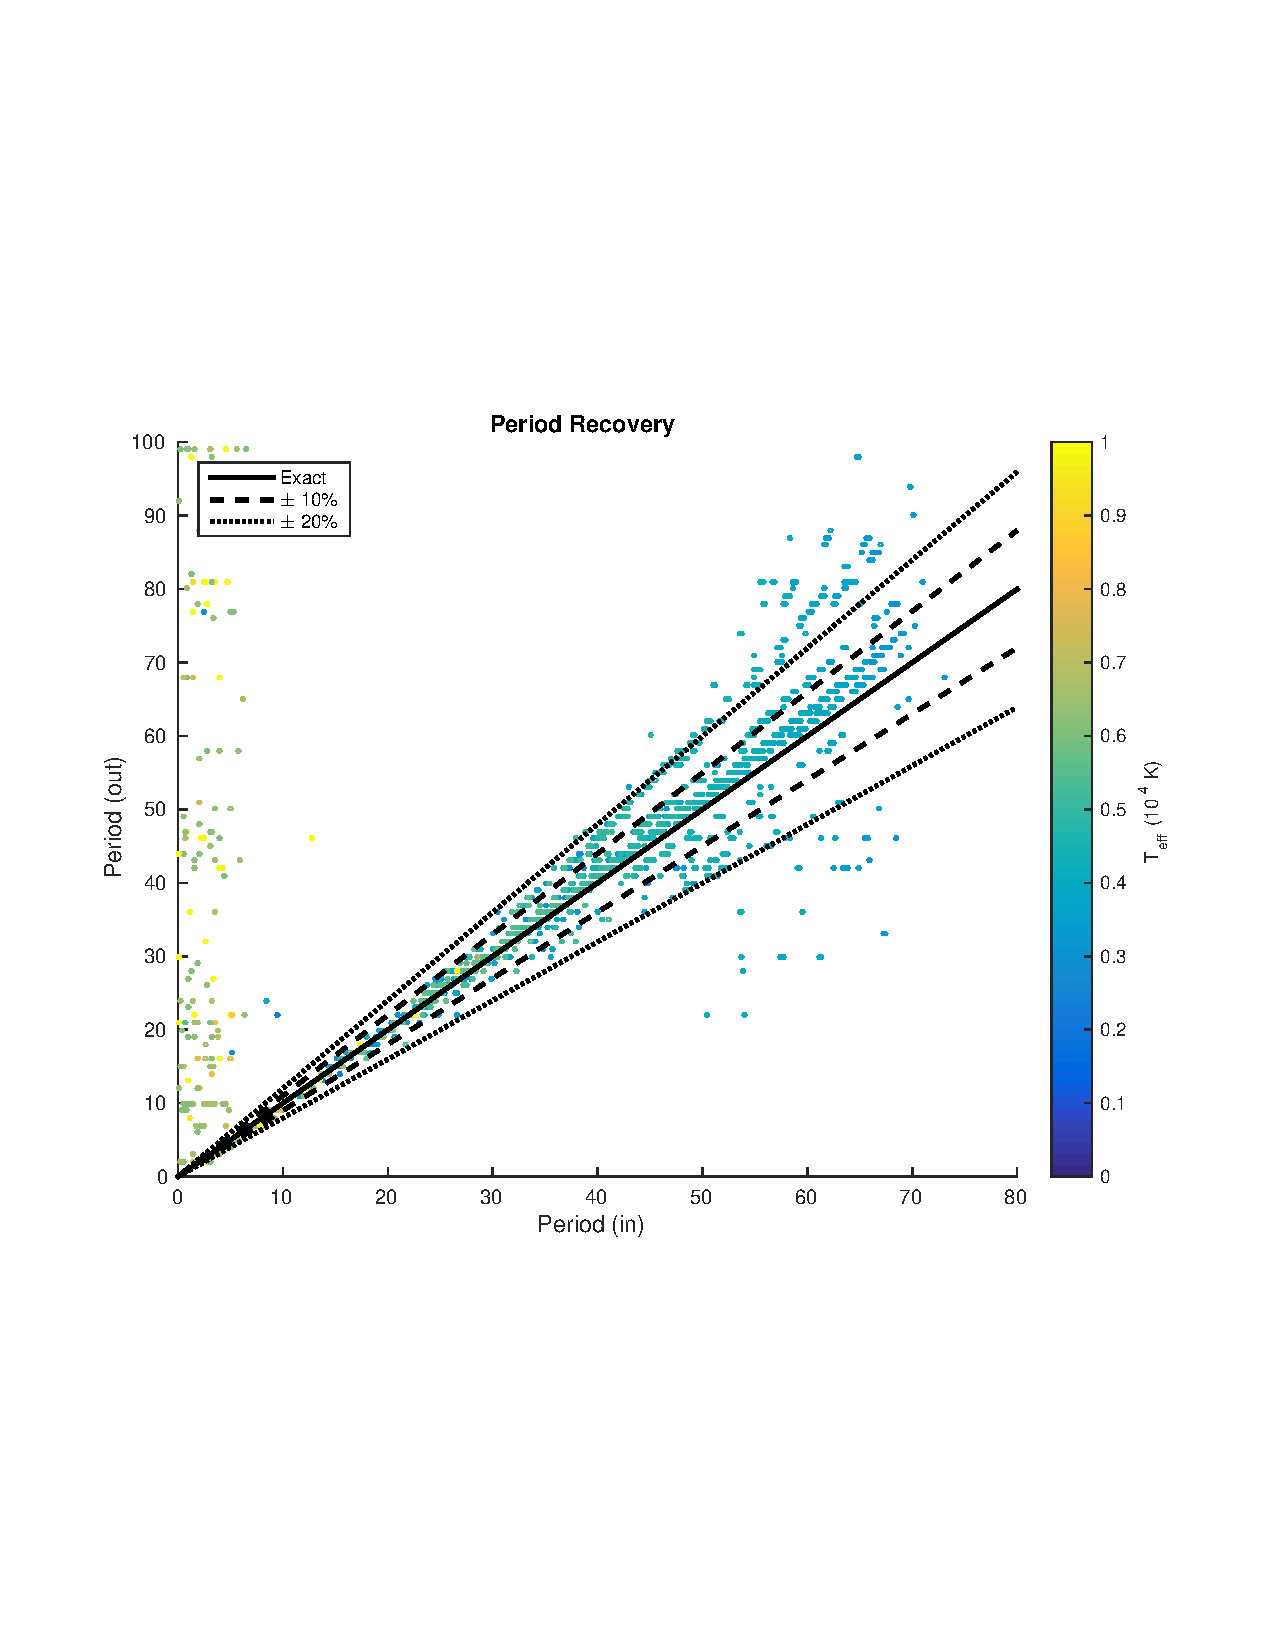
\includegraphics[width=6in, clip=true]{figures/figure6.pdf}
% \caption[\LSST\ rotation period recovery results.]
% {Measured versus injected rotation period for 5000 simulated \LSST\ targets.
% Points are coloured according to their temperatures.
% Rotation periods less than $\sim$ 10 days have a low recovery fraction, and
% this is worse for hot stars as they have lower amplitudes of variability.
% Figure made by Derek Buzazi.}
% \label{fig:derek}
% \end{center}
% \end{figure}

% \begin{figure}
% \begin{center}
% 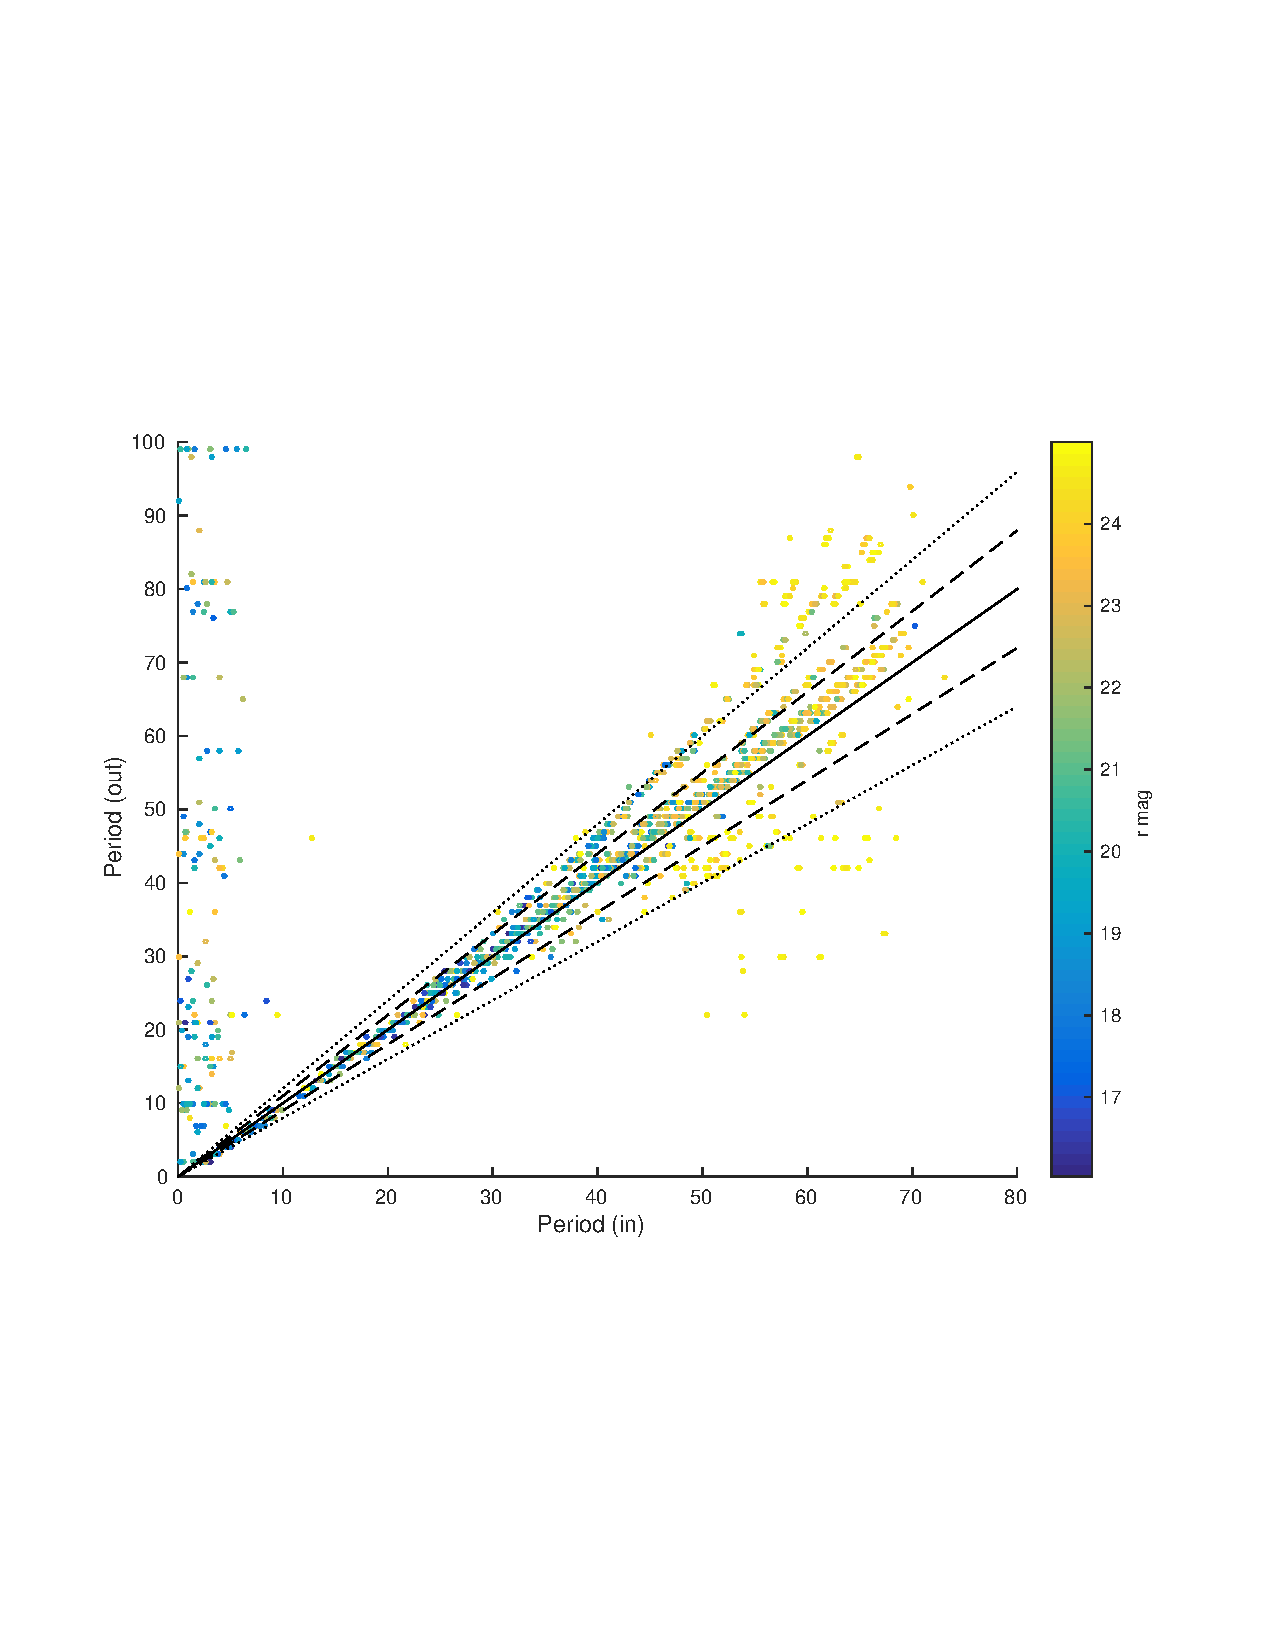
\includegraphics[width=6in, clip=true]{figures/figure8.pdf}
% \caption[\LSST\ rotation period recovery results.]
% {Measured versus injected rotation period for 5000 simulated \LSST\ targets.
% Points are coloured according to the $r$-band magnitude.
% The large outliers at long rotation periods are mostly faint.
% Figure made by Derek Buzazi.}
% \label{fig:derek2}
% \end{center}
% \end{figure}

% This work is the start of an ongoing effort to understand the opportunities
% for rotation period recovery in \LSST\ data.
% The next steps will be to estimate the total number of rotation periods we
% expect to measure from \LSST\ light curves and the types of stars we will be
% able to measure them for.
